\section{Results}\label{sec:results}

\paragraph{Data.} PsychAD prefrontal-cortex microglia and perivascular macrophages (CELLxGENE dataset 09642770, \NnucPsy{} nuclei, 1{,}469 donors, 10x 3$'$ v3) \citep{Lee2026}, three subtypes: Homeo\_CECR2 (\DPone{} donors with $\ge$4 nuclei, median \MedPone{} nuclei per donor), PVM\_CD163 (\DPtwo{}, median \MedPtwo) and ADAM\_GPNMB (\DPthree{}, median \MedPthree; 38\% of donors have fewer than 10). OneK1K blood \citep{Yazar2022}: transitional B (B1, 951 donors, median 20 cells), naive B (B2, 972, median 56) and naive CD4$^+$ T cells (B3, 981, median 244). For each cell type we test all pairs among the 400 most expressed genes plus sex-linked, heat-shock and perivascular control genes (87{,}990--89{,}676 pairs), with Benjamini--Hochberg (BH) at $q=0.05$ \citep{BenjaminiHochberg1995}. SEA-AD results are in Appendix~\ref{app:smallD}.

\paragraph{Real-cell nulls.} Reassigning the cells of one type at random to pseudo-donors that keep the real donors' cell numbers gives data with real within-cell programs, real depths and real cell-number imbalance, but zero between-donor covariance for every pair (\emph{pooled null}). Pooling turns real between-donor differences into within-pseudo-donor structure, so the \emph{donor-centred null} first divides out each donor's shrunken mean effect (Appendix~\ref{app:methods}). The \emph{bank-stratified null} reassigns donor-centred cells only among donors of the same brain bank, so pseudo-donors inherit their bank's depth and handling. Under a complete null every call is false, so the FDR equals the probability of at least one call per reassignment (run-level error); each frozen plan judged a method within bound if that fraction was at most $0.05+2$\,SE.

\subsection{Pseudobulk fails, and so do its corrections}\label{sec:null}

\begin{figure}[t]
\centering
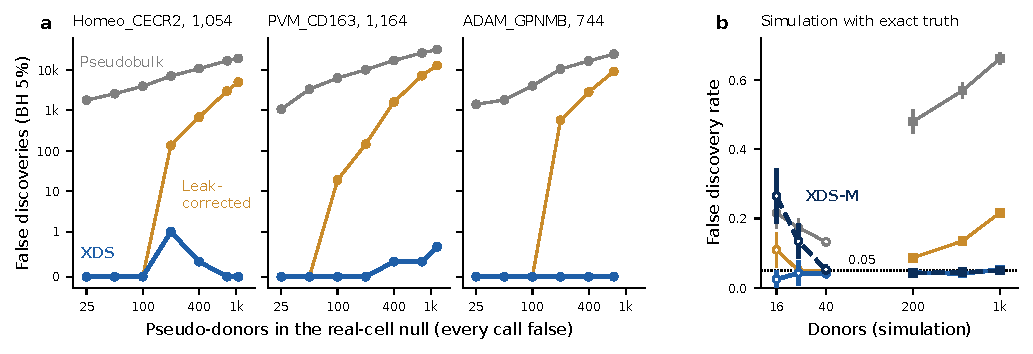
\includegraphics[width=\linewidth]{figures/fig_growth.pdf}
\caption{False discoveries grow with cohort size, and XDS-M controls them from about 100 donors. (a) Mean BH false calls on the PsychAD pooled null against the number of pseudo-donors (nested random subsets; three reassignments for $D\ge200$, one below; LCP and XDS shown from 200 up, as below that they had too few permutations to make a call; LCPd, KX and XDS-M not run); axes linear below 1, logarithmic above. (b) Reassignments with at least one false call on the donor-centred null, pooled over subtypes; bars, exact 95\% intervals. 25--100 pseudo-donors: 300 runs (REV3) for pseudobulk, XDS-M and KX, and \RfRoneN{} runs per subtype with $2\times10^6$ donor permutations (REV4) for LCP, LCPd and XDS (open circles); 200 to full size: 300 runs (REV2), normal references (filled).}
\label{fig:growth}
\end{figure}

On the donor-centred null at full cohort size, pseudobulk made \RfPBmean{} false calls per reassignment (20 per subtype; per-pair type-I error 0.23--0.37), and on the pooled null \PBnullCalls{}. The number grows with the number of pseudo-donors (Fig.~\ref{fig:growth}a), and on the pooled null \PBposFrac{} of the false edges are positive correlations, the sign of a factor shared by all genes, with median $|r|$ \FalseRmed{}. On the OneK1K pooled null, with medians of 20--244 cells per donor, pseudobulk made \RfOnekPB{} false calls per reassignment (Table~\ref{tab:pbfix}).

None of the standard repairs fixes it (Table~\ref{tab:pbfix}). Regressing each gene's log-CPM on log cell number and log depth (PBres) left \RfPBres{} false calls; removing the top 5 or 10 principal components of the donor-by-gene matrix, the usual correction for confounded co-expression \citep{Parsana2019}, left \RfPCadj{} in brain. Weighting donors by cell number (PBw) came closest: it left \RfPBwOne{} and \RfPBwThree{} false calls in Homeo\_CECR2 and ADAM\_GPNMB but \RfPBwTwo{} in PVM\_CD163, and \RfOnekPBw{} on the OneK1K pooled null (type-I \RfOnekPBwTI). Every reassignment of every variant made at least one false call. Leak-corrected tests fail too (Appendix~\ref{app:ablate}): subtracting an estimated leak with self-standardization (LCP) leaves the transformation bias and the error of the leak estimate (false calls in every run at 200 or more pseudo-donors); design-only standardization with leak subtraction (LCPd) fixes the transformation bias but not the estimation error; cross-splitting with self-standardization (LCPX) removes the leak but not the transformation bias; and an exact U-statistic correction (XU) has a depth--state coupling bias linear in the depth slopes (Proposition~\ref{prop:coupling}), where XDS's is quadratic (Lemma~\ref{lem:coupling}). Only disjoint cells together with design-only standardization remove all three biases.

\begin{table}[t]\centering\small\setlength{\tabcolsep}{4pt}
\caption{Pseudobulk and its corrections on real-cell nulls at full cohort size: mean BH false calls per reassignment (per-pair type-I error in parentheses); every reassignment of every variant made at least one false call. PsychAD: donor-centred null, 20 reassignments per subtype. OneK1K: pooled null, 10 reassignments per cell type (B1, B2, B3 as in the text). Variants as in Table~\ref{tab:methods}.}\label{tab:pbfix}
\begin{tabular}{lcccccc}\toprule & \multicolumn{3}{c}{PsychAD (donor-centred)} & \multicolumn{3}{c}{OneK1K (pooled)}\\\cmidrule(lr){2-4}\cmidrule(lr){5-7}
Method & Homeo & PVM & ADAM & B1 & B2 & B3\\\midrule
Pseudobulk & 12{,}685 (0.28) & 23{,}735 (0.37) & 8{,}566 (0.23) & 23{,}114 (0.38) & 22{,}556 (0.38) & 18{,}989 (0.35)\\
PBres & 8{,}576 (0.24) & 20{,}722 (0.34) & 6{,}483 (0.21) & -- & -- & --\\
PBw & 12 (0.02) & 4{,}820 (0.14) & 11 (0.02) & 1{,}096 (0.07) & 2{,}590 (0.12) & 2{,}050 (0.11)\\
PC5 & 8{,}690 (0.24) & 9{,}222 (0.25) & 5{,}018 (0.20) & 15{,}599 (0.31) & 17{,}974 (0.34) & 7{,}446 (0.23)\\
PC10 & 8{,}658 (0.24) & 8{,}879 (0.24) & 4{,}226 (0.19) & 13{,}355 (0.29) & 14{,}373 (0.30) & 4{,}084 (0.19)\\
\bottomrule\end{tabular}\end{table}


\begin{figure}[t]
\centering
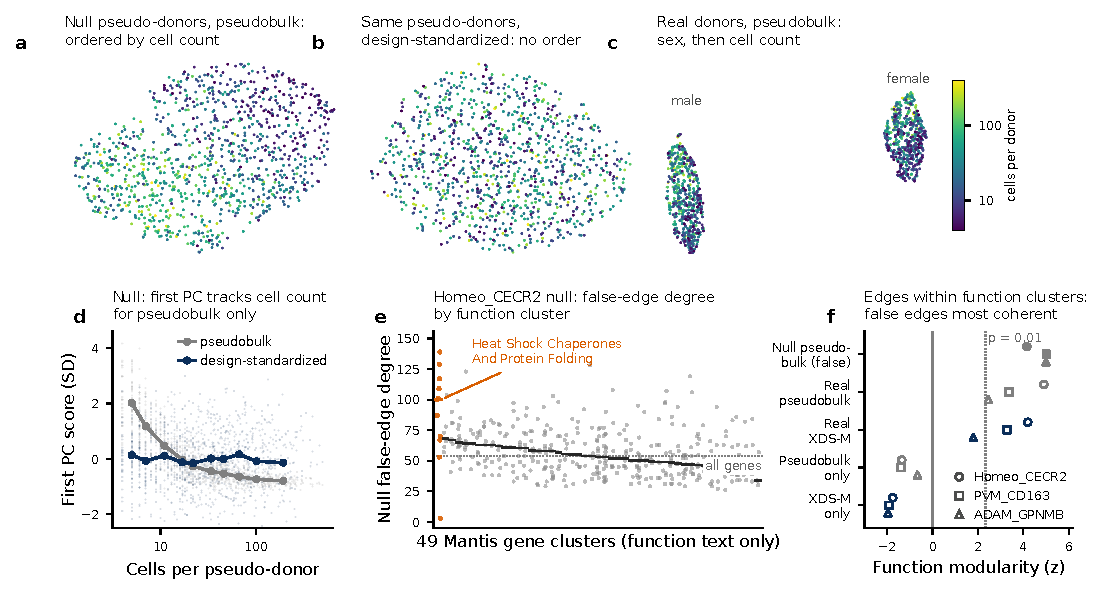
\includegraphics[width=\linewidth]{figures/fig_anatomy.pdf}
\caption{What a pseudobulk network is made of. Donor maps: our UMAP layouts; gene clusters: Mantis, from function text; all maps hosted in the Mantis space and redrawn here. (a) 1{,}054 Homeo\_CECR2 pseudo-donors of one donor-centred null reassignment (no between-donor co-expression), placed by UMAP of their pseudobulk log-CPM profiles and coloured by cell number. (b) The same pseudo-donors placed by their design-standardized full-donor profiles $R^*_{dj}$. (c) The 1{,}054 real donors, pseudobulk profiles: the two clusters are the donors' sex; colour, cell number. \GeneMapCaption{}}
\label{fig:anatomy}
\end{figure}

\subsection{What a pseudobulk network is made of}\label{sec:anatomy}

To see the artifact rather than count it, we built maps of donors and genes in Mantis, a semantic-mapping platform \citep{Mantis2026} (REV4 Amendment~1). We computed the donor layouts and every statistic; Mantis hosts the maps and supplies the gene map's layout and clustering from function text. Figure~\ref{fig:anatomy}a places the 1{,}054 pseudo-donors of one donor-centred Homeo\_CECR2 reassignment by UMAP \citep{McInnes2018UMAP} of their centred pseudobulk profiles. Nothing co-varies between these pseudo-donors, yet the map is ordered by cell count. The length of a pseudo-donor's profile has Spearman correlation \RsixNormPB{} with its cell number; the first principal component carries \RsixPConeVar{} of the variance, has loadings of one sign for \RsixPConeSign{} of genes, and has $R^2=\RsixPConeR$ with log cell number. This is the shared factor of Proposition~\ref{prop:transform} made visible: the log of a noisier mean is lower, so a few-cell donor's profile is pushed down for all genes at once (its mean log-CPM over genes correlates \RsixRowMeanLogn{} with log cell number), and every gene pair inherits a positive correlation through it. Laid out by their design-standardized donor values (the full-donor analogue of XDS-M's half-donor inputs), the same pseudo-donors show no order (Fig.~\ref{fig:anatomy}b; profile length versus cell number \RsixNormR, and $R^2\le\RsixPConeRR$ for each of the first five components). Real donors (Fig.~\ref{fig:anatomy}c) cluster by sex (2-means on the map agrees with recorded sex for \RsixSexConc), a true between-donor signal, and within each cluster are again ordered by cell count (second component $R^2=\RsixRealPCtwoR$); there the design-standardized profile length also tracks cell number (\RsixRealNormR), because cell number is associated with diagnosis and other donor traits (Section~\ref{sec:dc}). At the level of pairs, a pair's false pseudobulk correlation in the null tracks its within-donor cell-level correlation in real donors (Spearman \RsixPairNull{} over all pairs), the leak of Proposition~\ref{prop:leak}. \GeneMapText{}

\subsection{Calibration of XDS-M}\label{sec:calib}

\CalibText{}

\begin{table}[t]\centering\small\setlength{\tabcolsep}{3.2pt}
\caption{Run-level error on real-cell nulls: reassignments with at least one BH call, pooled over the three PsychAD subtypes (under a complete null this fraction is the FDR). $^\dagger$: outside the frozen bound ($0.05+2$\,SE) in at least one subtype or cell type. Donor-centred null: 25--100 pseudo-donors from REV3 (100 runs per subtype) for pseudobulk, XDS-M and KX, and from REV4 with $2\times10^6$ donor permutations (18--18 runs per subtype) for LCP, LCPd and XDS, which use permutation $p$-values at $D\le100$; 200 to full size from REV2 (100 runs per subtype, normal references). Bank: brain-bank-stratified null at full size (REV4, 40 runs per subtype); the bank-centred row is post hoc (Section~\ref{sec:calib}). OneK1K: pooled null at full size, three cell types (REV2; 30--33 runs each).}\label{tab:calib}
\begin{tabular}{lcccccc|c|c}\toprule & \multicolumn{6}{c|}{Donor-centred null, pseudo-donors} & Bank & OneK1K\\
Method & 25 & 50 & 100 & 200 & 400 & full & full & full\\\midrule
Pseudobulk & 300/300$^\dagger$ & 300/300$^\dagger$ & 300/300$^\dagger$ & 300/300$^\dagger$ & 300/300$^\dagger$ & 300/300$^\dagger$ & 120/120$^\dagger$ & 90/90$^\dagger$\\
LCP & 27/34$^\dagger$ & 17/34$^\dagger$ & 34/34$^\dagger$ & 300/300$^\dagger$ & 300/300$^\dagger$ & 300/300$^\dagger$ & 120/120$^\dagger$ & 89/90$^\dagger$\\
LCPd & 29/34$^\dagger$ & 6/34$^\dagger$ & 4/34$^\dagger$ & 46/300$^\dagger$ & 42/300$^\dagger$ & 68/300$^\dagger$ & 76/120$^\dagger$ & --\\
XDS, one split & 1/34 & 1/34 & 3/34$^\dagger$ & 97/300$^\dagger$ & 82/300$^\dagger$ & 81/300$^\dagger$ & 27/120$^\dagger$ & --\\
XDS-M & 147/300$^\dagger$ & 39/300$^\dagger$ & 15/300 & 9/300 & 23/300$^\dagger$ & 9/300 & 25/120$^\dagger$ & 6/99\\
KX & 300/300$^\dagger$ & 237/300$^\dagger$ & 67/300$^\dagger$ & 24/300 & 16/300 & 11/300 & 25/120$^\dagger$ & --\\
XDS-M, bank-centred & & & & & & & 7/120 & \\
\bottomrule\end{tabular}\end{table}


\paragraph{Single split versus studentization.} On the donor-centred null, single-split XDS made a false call in \RtwoRangeXDS{} of 100 runs per subtype and size, although its $p$-values are calibrated in bulk (\RoneXDSnfour{} below $10^{-4}$ per run against \RoneExpnfour{} expected), consistent with a normal reference that is too light in the extreme tail where BH makes its first call; a direct check at 200 pseudo-donors with $2\times10^6$ permutations was inconclusive (\PermTwoXperm{} against \PermTwoXnorm{} runs; Amendment~3). Studentizing by the donors' own spread corrects this: in a tail check with 2{,}000 genes (frozen plan REV3, A2), XDS-M with one split met the calibration rule in \AtwoHiDecMone{} stratum, null and size combinations and with five splits in \AtwoHiDecM, against \AtwoHiDecS{} for single-split XDS. Averaging over splits mainly stabilizes the call set (seed-to-seed Jaccard \RealXDSMjac{} on real donors; one split 0.67--0.83); with donor-specific overdispersion violating (A5) in simulation, XDS-M kept FDR \FtwoFDRXDSM{} and \FfiveFDRXDSM{} at 200 and 500 donors.

\paragraph{Expression level and blood.} With the 2{,}000 most expressed genes of OneK1K B1 and B2 (REV3, A2), XDS-M's observed-to-expected tail ratios at $p\le10^{-4}$ and $10^{-5}$ were \AtwoHiFourM{} and \AtwoHiFiveM{} for genes above 0.1 UMI per cell (rule met in \AtwoHiDecM) and \AtwoLoFourM{} and \AtwoLoFiveM{} at 0.03--0.1 UMI among B1 genes ranked 2{,}001--3{,}000 (rule met in \AtwoLoDecM), so we validate XDS-M above about 0.1 UMI per cell (ADAM\_GPNMB, 2{,}000 genes: \AtwoPthreeDecM; pseudobulk none). On the OneK1K pooled null (33 runs per cell type) XDS-M made a call in \OnekEanyXDSM{} runs, within the bound in all three cell types (the first 30 B1 runs alone, 4 of 30, exceed it).

\subsection{Power in simulations with exact truth}\label{sec:sim}

Real-cell nulls measure only errors, so power comes from a simulator with exact truth on the latent scale (80 genes; within-only, between-only and mixed programs, weak nulls; Appendix~\ref{app:sim}, Table~\ref{tab:sim}). With a median of 20 cells per donor, pseudobulk's FDR rose from \LPBFDRa{} at 200 donors to \LPBFDRc{} at 1{,}000 and LCP's from \LLCPFDRa{} to \LLCPFDRc{}, as Proposition~\ref{prop:growth} predicts, while XDS-M stayed at 0.043--0.050 with power \XDSMLpow{} at 200 donors (XDS \XDSLpowTwo; LCP 0.98 at FDR \LLCPFDRa). With strong depth--state coupling, XDS kept FDR \CoupleXDS{} at 200--1{,}000 donors, whereas the U-statistic test rose to \CoupleXU{} and pseudobulk to \CouplePB{}. In small designs XDS kept FDR at \SXDSFDRrange{} but had little power (\SXDSpowDforty{} at 40 donors with $\sim$40 cells; LCP \SLCPpowDforty, but LCP fails on real cells, Section~\ref{sec:calib}).

\subsection{False differential co-expression between AD cases and controls}\label{sec:dc}

\DCtext{} On the donor-centred null with AD labels kept (frozen plan REV2, extended to 20 reassignments per subtype in REV4), pseudobulk differential co-expression made on average \RfDCPB{} false calls per reassignment (subtype means), with at least one in every run. Centring within groups keeps mean differences between cases and controls out of the test, and leaving the per-donor products unstandardized (XDS-Mgu, REV2 Amendment~1) makes their mean the between-donor covariance whatever the cell number; XDS-Mgu made a false call in \RfDCgu{} of 20 runs per subtype, the standardized XDS-Mg in \RfDCg{}. On real donors XDS-Mgu called \DCrealU{} pairs (pseudobulk \DCrealPB), and in simulations with true differences its FDR was \DCtwoFDRU{} against \DCtwoFDRPB{} for pseudobulk (Appendix~\ref{app:dc}). Cases and controls also differ in age, sex and tissue handling, so these are associations, not effects of disease.

\subsection{Real donors}\label{sec:real}

On real PsychAD donors between-donor co-expression is dense: XDS-M called \RfRealXDSM{} pairs in the three subtypes (\RealXDSMfrac{} of pairs), stable across split seeds and replicated in independent halves of the donors (\RealXDSMrep{} of calls). As a positive control, XDS-M and pseudobulk both found all 7 \emph{XIST}--Y-linked pairs negative in every subtype (XDS-M $p\le\PosXYmaxpM$) and all 21 Y--Y pairs positive. Pseudobulk called \RfRealPB{} pairs, fewer than XDS-M in \RfPBfewer: on dense real signal both tests saturate, and the artifact shows in which pairs are called rather than in how many. \RfRealPBonly{} pseudobulk calls (\RfRealPBonlyPct) were not made by XDS-M. On the same donors, XDS-M's 5{,}000 strongest pairs and 20 highest-degree genes barely change between split seeds (\OvSeedTop{} and \OvSeedHub{} of 20 shared), whereas pseudobulk and XDS-M share \OvPBXTop{} and \OvPBXHub; this difference is no larger than that between two independent halves of the donors (XDS-M \OvHalfXTop{} and \OvHalfXHub, pseudobulk \OvHalfPBTop{} and \OvHalfPBHub; REV4 Amendment~3). Pseudobulk-only calls were not enriched for pairs called falsely in the matched null (odds ratios \OvORall), so on real donors we could not attribute specific edges or hubs to the artifact beyond split-half noise; its demonstrated consequences are lost error control under nulls and false group differences (Section~\ref{sec:dc}). \CoRealText{} XDS-M is thus a calibrated building block for covariate-adjusted analyses, not a network method by itself.

\section{Discussion}\label{sec:disc}

Treating the donor as the unit of replication is necessary but not sufficient for valid between-donor co-expression: a per-donor summary must have an expectation that does not depend on the donor's cell number, and the two genes of a pair must not be measured on the same cells. Pseudobulk violates both, and with tens of cells per donor this produces thousands of false edges that replicate, grow with the cohort, look functionally coherent, and confound comparisons between groups with different cell numbers.

\paragraph{Recommendations.} Pseudobulk correlation should not be used to test between-donor co-expression: on every real-cell null we built, in brain and in blood (pooled null) with medians of up to 244 cells per donor, it and every pseudobulk repair in Table~\ref{tab:pbfix} made false calls in every run. \RecText{} Any method can be checked with the pooled or donor-centred null, which needs only cells and donor labels.

\paragraph{Limitations.} \LimText{}

\paragraph{Availability.} Code, hashed plans, results and map tables: [public repository URL]; maps: \href{https://mantis.csail.mit.edu/space/f14d0b39-bc65-4fbc-996f-11b222365984}{Mantis space f14d0b39} (full link in Appendix~\ref{app:mantis}); data: CZ CELLxGENE \citep{CZICellxGene2025}.
